形式手法を強く推奨する理由には、
理論的根拠と経験的根拠がある。
以下の節で、それぞれを説明する。

\section {理論的根拠}
	\index{りろんてきこんきょ@理論的根拠}

	形式手法を強く推奨する理論的根拠は、以下の3つである。

\begin{itemize}
\item プログラムは数学系だから
	\index{ぷろぐらむはすうがくけい@プログラムは数学系}

	プログラムは元来、数学的に厳密な体系で定義された一つの数学系である。
	しかも、C++やJavaのプログラムは「検証が困難な数学系
	\footnote{変数への値の代入などの破壊的代入を行うので、
	「同じ条件を与えれば必ず同じ結果が得られ、他のいかなる機能の結果にも影響を与えない」
	という参照透過性を保つことができない。}
	」であることが分かっている。
	これに対して、形式手法は「検証が容易な数学系」をもとにしている。
	したがって、検証しやすい数学系で記述した方が品質を上げやすい。
	


\item 形式手法では、上流工程で仕様を検証可能だから

	要求分析工程
	\index{ようきゅうぶんせきこうてい@要求分析工程}
	\footnote{ユースケース記述などを作成する要求収集(Elicitation)工程の出力を解析し、
	厳密な仕様を記述し、その妥当性確認(validation)と正当性検証(verification)を行う工程。
	本ブックレットでは、要求工学が対象とする工程、あるいは要件定義と称する工程は、要求収集工程と見なす。}
	からプログラミング工程までのどこかで、数学系に変換しなければならない。
	いずれどこかの工程で数学系にするならば、なるべく早い工程、
	すなわち上流工程で数学系にしておいたほうが、
	下流工程から上流工程への手戻りが減り、プログラムの質だけでなく、開発の生産性も向上する。
	そして、形式手法は上流工程での検証を支援する。

	要求分析工程での欠陥修正コストを1とした時の、その他の工程での欠陥修正コストを示したものが、
	図\ref{fig:RelativeCost}である。
		\footnote{Source: Barry Boehm: “EQUITY Keynote Address”, March 19th, 2007}

	\begin{figure}[h]
		\centering
		{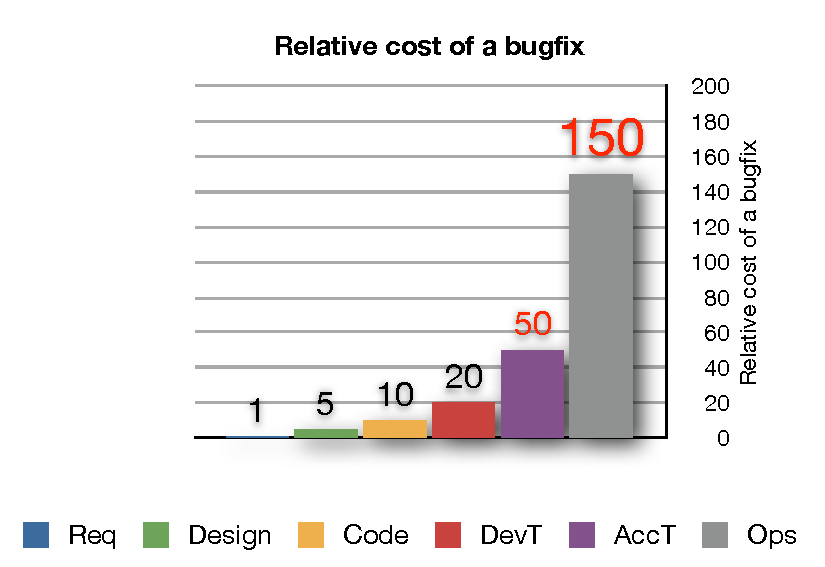
\includegraphics[width=40zw, keepaspectratio] {./Chapter1/image/RelativeCost.pdf}}
		\caption{開発工程別の欠陥修正コスト}
		\label{fig:RelativeCost}
		\index{かいはつこうていべつのけっかんしゅうせいこすと@開発工程別の欠陥修正コスト}
	\end{figure}

	このグラフから分かるように、上流工程での欠陥修正コストは、下流工程のそれの5分の1から150分の1にもなる。

	ここで、横軸のReq, Design, Code, DevT, AccT, Opsは、
	それぞれ要求分析、設計、コーディング、開発テスト、受入テスト、運用の各工程を示している。
	開発テストはシステム開発者によるテスト、受入テストはシステム発注者によるテストである。

\item 旧来の手法では、検証が困難だから

	旧来の手法では、レビュー以外の検証手段が無いため、
	中規模以上のシステムの検証は非常に困難であり、
	大規模システムの検証は不可能といっても良いほどの困難を伴う。

\end{itemize} 


\section {経験的根拠}
	\index{けいけんてきこんきょ@経験的根拠}

	形式手法による仕様記述を行った経験から分かったことは、以下の2点である。

\begin{itemize}
\item 日本語で「正しい」仕様を書くのは「不可能」である

	\begin{itemize}
	\item 曖昧さの排除が困難

		自然言語による仕様では、曖昧さの排除が困難である。

	\item ツールによるチェックが、ほとんど不可能

		自然言語で書かれた仕様を、ツールによってチェックすることはほとんどできない。
		これは、自然言語の文法定義と意味定義が曖昧なことによるもので、
		どのようなツールを作っても、曖昧さを排除することはできない。
		
		これに対し、形式手法で使用される形式仕様記述言語は、
		文法定義・意味定義ともに厳密であり、曖昧な仕様を書くことはできない。

		実際に、\ref{VDMeffect}章で示す成功例では、ツールによる静的検証
		\footnote{モデルを動かさずに検証すること}によって、
		ほとんどの単純ミスを検出し、
		動的検証
		\footnote{モデルを動かして検証すること}によって、
		すべての欠陥を検出し、修正することに成功した。

	\item 仕様の修正に弱い
		\index{しようのしゅうせいによわい@仕様の修正に弱い}

		自然言語仕様の検証は、主としてレビューに頼っているため機械化できない。
		これに対して形式手法は、形式仕様記述言語で書かれた仕様を、機械的に検証する手段を持っている。
		
		\ref{VDMeffect}章で示す成功例では、「仕様修正に強い」形式手法の利点が、品質向上と検証工数削減に大いに役立った。
		
	\item その場で「文法」を考えなければならない

		日本語で仕様を書ききれなくなり、if文などを使った擬似コード的な仕様を書くことが多く、
		擬似コードの文法
		\index{ぎじこーどのぶんぽう@擬似コードの文法}
		を考えている時間が馬鹿にならない。
		すなわち、仕様を書く際に、仕様の意味ではなく、文法に注意が向いてしまい、
		肝心な「意味を考える」ことがおろそかになってしまう。

	\end{itemize} 

\item 形式手法の方が技術移転や蓄積が容易である

	\begin{itemize}
	\item 日本語による意思疎通は難しい
		\index{にほんごによるいしそつう@日本語による意思疎通}


		日本語仕様は、開発者間のコミュニケーションを経るたびに、
		一種の伝言ゲームになってしまい、当初の意味がずれていくことが多い。
		打ち合わせなどで「あれって、こういう意味じゃないの」というような議論が起こることが多ければ、
		それは、自然言語の曖昧さによって意思疎通がうまくいっていない事の証である。

	\item 仕様記述言語を読むのは容易である
		\index{しようきじゅつげんごをよむのはようい@仕様記述言語を読むのは容易}

		自然言語仕様であろうが、形式仕様であろうが、仕様を書くことは難しい。
		しかし、記述された仕様を読むことは、形式仕様記述言語の場合、容易である。
		それは、非形式的な図形言語UML1.xより容易であり、UML2.0より遙かに簡単である。
		\index{UML@UML}

	\item フレームワークやライブラリの構築が容易である
		\index{ふれーむわーくやらいぶらりのこうちくがようい@フレームワークやライブラリの構築が容易}

		形式仕様記述言語は、プログラミング言語などと同じように、
		フレームワークやライブラリの構築が容易であり、
		再利用性や保守性に優れている。

	\item 業務知識の蓄積も容易である
		\index{ぎょうむちしきのちくせい@業務知識の蓄積}


		ExcelやWordによる自然言語仕様と異なり、形式仕様記述言語の仕様は通常テキストファイルであり、
		プログラミング言語と同じように、版管理や構成管理ツールと連動して容易に管理できるため、
		業務知識をいったん形式仕様記述言語で記述できれば、
		それを、再利用・保守可能な業務知識として、蓄積していくことが容易である。
	
	\item 仕様を「動かしてみる」ことができるので、理解しやすい
		\index{しようをうごかす@仕様を動かす}
		形式手法は、形式仕様を動かす(実行する\footnote{仕様アニメーションという}、
		モデル検査する、証明する)ことが可能で、
		動かない旧来手法より理解することが容易である。
	\end{itemize} 
\end{itemize} 


\section {日本語仕様の曖昧さの例}
	\index{にほんごしようのあいまいさのれい@日本語仕様の曖昧さの例}

	この節では、著者が出会ったことのある、日本語仕様の曖昧さの例を示す。

\subsection {図書館の本}
	\addcontentsline{toc}{section}{図書館の本}
	\index{としょかんのほん@図書館の本}

	図書館のシステムを考えた場合、以下の2つの文に出てくる「本」は同じものを意味しているだろうか?

\begin{itemize}
	\item 題名で本を検索する
	\item 本を図書館の蔵書として追加する
\end{itemize} 

	この2つの「本」は同じ場合もあるが、
	普通は、異なるものを指す。

	「題名で本を検索する」場合の「本」は、多くの場合、ある著者が書いたある題名の「本」を指す。
	この「本」は抽象的な概念で、例えばこの「本」が1000部出版されているとしても、我々は「ひとつの本」として認識している。

	しかし、図書館の蔵書に追加する「本」はそうではない。
	これは物理的な1冊の本であり、抽象的な「本」が1000部出版されていれば、こちらの「物理的な本」は1000冊存在する。

	日本語による仕様記述では、このように区別すべき用語が同じものとして記述されたり、
	同じ意味の用語が別の言葉で記述されて曖昧さが混入し、開発者同士のコミュニケーションが混乱し、
	結果として、作業の手戻りの多発による生産性の低下と品質の低下を招く。

	詳細は、\ref{LibraryModel}章を参照していただきたい。

\subsection {特急券予約システム}
	\addcontentsline{toc}{section}{特急券予約システム}
	\index{とっきゅうけんよやくしすてむ@特急券予約システム}

	ここでは、筆者が実際に遭遇した、鉄道会社Aの特急券予約システムの問題点を紹介する。

	問題の発端は、クレジットカード会社の都合で、
	特急券予約システムに使用していたクレジットカードを変更せざるを得なくなり、
	特急券予約システムの設定を変更しようとしたところから始まった。

	以下は、鉄道会社Aサポートセンターとの問答である。
	\footnote{実際にあった事例をかなり省略している。}

\begin{enumerate}
\item 客(すなわち筆者)は、おサイフケータイ(鉄道会社B)で特急券予約システム(鉄道会社A)を使っていた。
\item 会社Cクレジットカードが廃止になり会社Dクレジットカードに変更して下さいとの連絡があった。
\item 鉄道会社Aサポートセンターに電話したところ、
	おサイフケータイの登録クレジットカードを変更すれば、2日後には特急券予約システムが使えますとのことだった。
\item おサイフケータイの設定でクレジットカードを変更し、2日後に使おうとしたが、特急券が予約できなかった。

\item 予約できなかったので鉄道会社Aサポートセンターに電話した

	\begin{description}
	\item [客]「クレジットカードを変更したら、予約できないんですが?」
	\item [鉄道会社A]「カードを変更したら、新規に特急券予約システムを契約して下さい。」
	\item [客]「クレジットカード変更前に予約した特急券に引き換えようとしたらできないのですが?」
	\item [鉄道会社A]「カードで引き替えできるようになったので、それで引き換えて下さい。暗証番号はカードのものを使って下さい。」
	\item [客]「カードの暗証番号って、何ですか?」
	\item [鉄道会社A]「クレジットカードの暗証番号です。」
	\end{description}

\item 旅行当日のT駅での問答

	\begin{description}
	\item [客]「クレジットカードで特急券に引き換えできないんですが?」
	\item [鉄道会社B]「会員証でやってみて下さい。」
	\item [客]「会員証でもできないんですが?」
	\item [鉄道会社B]「変ですねー、こちらでやってみましょう。駄目ですねー...」
	\item [客]「ひょっとして、古いクレジットカードでは駄目ですか?」
	\item [鉄道会社B]「あ、できましたね。はい、切符です。」
	\end{description}
\end{enumerate}

	上記のやり取りで、何が起こっていたかを正確に理解できる方は居るだろうか?
	理解できるはずはない。
	鉄道会社A側の用語の使い方が適切ではないので、
	鉄道会社Aサポートセンターの要員も、T駅の鉄道会社Bの駅員も事態を正確に把握できなかったのだから。

その後、手元にある特急券予約システム関係のカード類と、インターネット上の情報と、
鉄道会社Aサポートセンターへの何回かの電話によって、幾つかの用語の定義、すなわちカードの種類が判明した。

すなわち、

\begin{itemize}
	\item 予約会員証 (変更前、変更後)、クレジットカード(変更前、変更後)
	\item おサイフケータイ
		\footnote{ここでは、スマートカードとして特急券を予約する機能だけに着目する。}
	\item ICカード、予約カード
\end{itemize} 

このうち、ICカードはおサイフケータイで予約する場合には関係ないカードであることが判明した。
また、予約カードも鉄道会社Aのカードであり、
おサイフケータイ(鉄道会社B)から特急券予約システムする場合には関係ないことも判明した。

これらを反映して、最初の鉄道会社A側とのやり取りを、正確な用語で記述すると以下のようになる。

\begin{enumerate}
\item 予約できなかったので鉄道会社Aサポートセンターに電話した

	\begin{description}
	\item [客]「クレジットカードを変更したら、予約できないんですが?」
	\item [鉄道会社A]「クレジットカードを変更したら、新規に特急券予約システムを契約して下さい。」
	\item [客]「クレジットカード変更前に予約した特急券に引き替えようとしたらできないのですが?」
	\item [鉄道会社A]「予約会員証で引き替えできるようになったので、それで引き換えて下さい。
			暗証番号はクレジットカードのものを使って下さい。」
	\end{description}

\item 旅行当日のT駅での問答

	\begin{description}
	\item [客]「変更後のクレジットカードで特急券に引き換えできないんですが?」
	\item [鉄道会社B]「予約会員証でやってみて下さい。」
	\item [客]「予約会員証でもできないんですが?」
	\item [鉄道会社B]「変ですねー、こちらでやってみましょう。駄目ですねー...」
	\item [客]「ひょっとして、変更前のクレジットカードでは駄目ですか?」
	\item [鉄道会社B]「あ、できましたね。はい、切符です。」
	\end{description}
\end{enumerate}

この記述は、VDM++という形式仕様記述言語を使って、前記の問答に関わる仕様(モデル)
\footnote{詳細は、\ref{How2MakeModel}章と、\ref{EvolvedExpressReservation}章を参照のこと。}
を書き、
最初の問題発生から3ヶ月かかって、問題を解決した後に記述したものである。


\subsection {応当日}
	\addcontentsline{toc}{section}{応当日}
	\index{おうとうび@応当日}

以下は、証券会社用のパッケージソフトウェアを作成していた際、
「信用取引の決済日」の定義を聞いた時に回答として得た説明文章である。

\begin{itemize}
	\item 信用取引の決済日(期日)を得る。

	弁済期限とは、信用建玉に対して当社がお客様に信用を供与する期限をいいます。
	弁済期限は、現在のところ6ヶ月のみを取扱っています。
	弁済期限が6ヶ月であるということは、
	信用建玉の建日(信用建玉が約定した日)の6ヶ月目応当日が信用期日となり、
	この日を超えて建玉を保有することは法律で禁じられています。
	信用期日が休日の場合には、直近の前営業日が信用期日となります。
\end{itemize} 

直ちに生じる疑問は、以下のようなものであろう。

\begin{itemize}
	\item 弁済期限と決済日と信用期日との関係は?
	\item 応当日とは何か?
\end{itemize} 

弁済期限と決済日と信用期日との関係を質した所、直ちに回答が得られた。
すなわち、これらは同一である。

応当日については、何回かのやり取りの後、以下の回答が得られた。

普通の日本語で書くと分かり難くなるので、
やや形式化した日本語で応当日を「曖昧に」定義すると、以下のようになる。

\begin{verbatim}
現在日をy年m月d日としたとき、nヶ月後の応当日とは、y年m+n月d日のこと。

ここで、m+n >= 13 ならば、
   年候補Yをy + (m+n - 1) div 12とし、
   月候補Mをm+n mod 12として、
      Mが0ならば、Mは12、
      Mが0以外ならば、Mをそのまま使って、
Y年M月d日が応当日である。
ここで、divは整数の除算、modは整数除算の余りを得る演算子である。
\end{verbatim}

この日本語仕様には、まだ、以下の問題が残っている。

\begin{enumerate}
\item たとえば信用建玉の建日が8月31日だと、応当日は翌年2月31日になってしまうのだが、
	そのとき2月28日あるいは2月29日にするのか3月1日にするのかの記述がない。
\item 応当日から月初日まですべて休日の場合、前月の営業日にしてよいのかどうかの記述がない。
\end{enumerate}

この疑問は、証券業務の専門家に質問したところ、半日ほどで回答を得た。

\begin{itemize}
	\item 月末日を越えたら、月末日に最も近いその月の営業日。
	\item 応当日が休日で、前営業日が前の月の場合、その営業日が応当日になる。
\end{itemize} 

以上のように、「信用取引の決済日を得る」という証券業務にとっては基本的な用語すら、
同じ事を表す複数の言葉が存在し、定義が曖昧で、
ある程度の仕様分析を行った後、
証券業務の専門家に質問しても答えを得るのに半日以上を要して
ようやく正しい仕様を理解できた。

しかも、応当日の年や月を求める計算は、日本語で記述し理解するには複雑すぎる。

これでは、生産性と品質が悪くなるはずである。
